%%%%%%%%%%%%%%%%%%%%%%%%%%%%%%%%%%%%%%%%%%%%%%%%%%%%%%%%%%%%%%%%%%%%%%%%%%%%%%
%%Skeleton LaTeX file: double column format.
%%%%%%%%%%%%%%%%%%%%%%%%%%%%%%%%%%%%%%%%%%%%%%%%%%%%%%%%%%%%
%%REMEMBER THAT THERES IS AN EIGHT PAGE SIZE RESTRICTION
%%%%%%%%%%%%%%%%%%%%%%%%%%%%%%%%%%%%%%%%%%%%%%%%%%%%%%%%%%%%

%%% Sample file for ME Project Papers for Evaluation by Supervisor and Reader

\documentclass{article}

\usepackage{multicol}

\usepackage[none]{hyphenat}		%prevent breaking of words

\usepackage{graphicx} 
\pagestyle{empty}
\setlength{\topmargin}{ 0.25in}
\setlength{\columnsep}{2.0pc}
\setlength{\headheight}{0.0in}
\setlength{\headsep}{0.0in}
\setlength{\oddsidemargin}{-.19in}
\setlength{\parindent}{1pc}
\textheight 8.75in
\textwidth 6.8in

\title{\large \bf A method to mitigate the Code-Reuse Attacks }
\author{Niranjan Singh}

\date{May 16th, 2016}

\begin{document}

	\maketitle
    \begin{center}
        ME Project Final Report
    \end{center}
        \vskip 12pt
	\thispagestyle{empty}
	\bibliographystyle{unsrt}
	
		\begin{abstract}
		Code-reuse attacks are one of the dominant security exploits present today. They don't need any malicious code injection instead they uses the code present in the address space of the process by directing the control flow to the attackers payload. These are shown to be Turing-complete i.e.,they can cause arbitrary execution. Many mitigation techniques have been proposed from time to time to prevent these attacks but no one is a full proof solution they can be bypassed in one or the other ways. Some methods like stack canary, Dynamic execution prevention, code randomisation were proposed but shown to be bypassed. This lead to the development of new offensive approaches like Just-in-time code reuse, and solutions like HAFIX.
		
		In our work, we propose a method of mitigation of the code-reuse attacks that would prevent the discloser of a gadget called stack pivot sequence which is important for a code-reuse attack to succeed. These probable stack pivot sequences are replaced with some other valid code and encrypted, and are replaced back upon execution. It successfully prevents the discovery of stack pivot sequences, thereby preventing attack on an executable offline. However, applying this method at runtime requires much more support.
	\end{abstract}	
	
	\hfill \\
	
	\begin{multicols}{2}
	\section{INTRODUCTION}
	Memory corruption vulnerabilities are one of the oldest and most exploited vulnerabilities. One of the main reasons being the insecure coding practices and omitting the security features like strong typing, bounds checking, etc. in legacy code to provide better efficiency. And for a long time these vulnerabilities have been exploited by the attackers for malicious purposes.

	Starting from the buffer overflow vulnerabilities that allowed the attacker to put some payload on stack and redirect execution to it \cite{aleph}. The payload is used for malicious activities like getting a remote shell. It motivated security researcher to focus on these vulnerabilities and some solutions were proposed. The StackGuard compiler addressed this stack smashing by checking the integrity of activation records by putting a "canary" word next to return address on stack \cite{stackguard}. Some other techniques also came into existence like address space layout randomisation(ASLR) \cite{pax} that randomises the address space of the executable, and Data Execution prevention(DEP) that prevent the execution of code by preventing memory pages being both writeable and executable at the same time. But some methods started coming up to bypass these security methods. G. Richarte et al. \cite{4trick} presented four tricks to bypass the stack samashing protection provided by StackGuard. The ASLR protection can be bypassed by brute force \cite{effaslr}. DEP can be bypassed by Return Oriented Programming(ROP). The code-reuse  attacks came in practice that instead of inserting new code, reuses the present executable code to perform operations they need. And some more methods were proposed like fine-grained ASLR, control flow integrity(CFI) checking, and even hardware based solutions like HAFIX \cite{hafix}. But, some new attacks came like Just-in-time ROP that bypasses fine-grained ASLR \cite{jitrop}, and some also showed bypassing of CFI solutions. Also, ROP is Turing-complete i.e., it can perform an arbitrary execution. This, emphasises on the need of more work in the field.
	
	The focus of our work would be mitigate code-reuse attacks by preventing the exposure of stack pivot sequence(explained in section 2.2) to attackers.
	
	\section{Background}
	
	\subsection{Buffer Overflow}
	Applications use call stack for execution of the subroutines. It stores the state of a subroutine in form of activation record(stack frame) when control is passed on to some other subroutine. It stores the parameters of the callee, return address, frame pointer, and local variables. The structure of call stack is shown in figure below.
	
	\
	\
	
	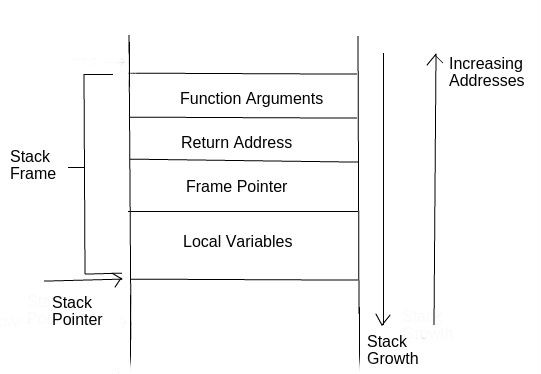
\includegraphics[scale=.4]{stack_normal.jpg}
	\
	\
	\
	
	Consider a small C language subroutine with one local variable "buffer" of size 12 bytes. If the argument passed is more than the buffer can hold, strcpy() does not check the bounds and directly copies, thereby overwriting the locations next to buffer, i.e.,the frame pointer and eventually the return address, this is termed as overflowing the buffer. By crafting a specific input the buffer can be overflown and the return address can be overwritten to direct the control flow to the attackers payload. 
	
	Say the shellcode to execute a shell is placed by the attacker on the stack at address 0$\times$80484cd, it can be done by passing the shellcode as the argument which would be then stored on the stack. By passing a input like "A"*12 +"A"*4 +"\textbackslash $\times$cd\textbackslash $\times$84\textbackslash $\times$04\textbackslash $\times$08", the first 12 bytes will fill the buffer variable, the next 4 will overwrite the frame pointer, and the others will overwrite the return address by 0$\times$80484cd. And stack looks like this
	
	\
	\
	\
	
	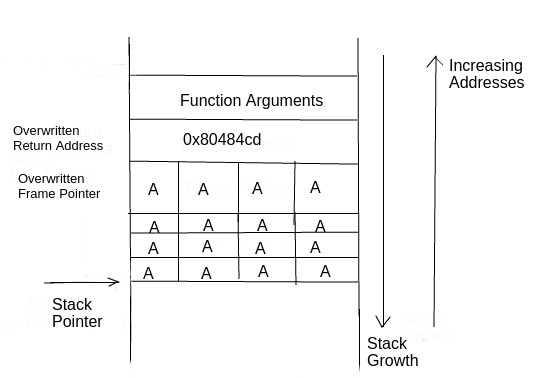
\includegraphics[scale=.45]{stack_prog.jpg}	
	
	When this subroutine returns the address 0$\times$80484cd will be popped in the instruction pointer to start execution from that address thereby executing the malicious code injected by the attacker\cite{aleph}.
	
	But, this code injection was easily prevented by Data execution prevention(DEP) technique, which is deployed in almost every OS today. DEP marks area as "executable" or "non-executable". This is also called W$\oplus$X protection, it prevents a memory page from being writeable and executable at same time. Thus, the code inserted by the attacker in stack or heap segments can not be executed thereby preventing code injection. It is enforced by hardware(NX or XD bit) and also by software. But, Attackers found ways around it and started using the code present in the libraries loaded along with executable and even the code present in the executable to construct the payload, thereby giving rise to code-reuse attacks.
	
	\subsection{Code-Reuse Attacks}
	Code-Reuse attacks are the software exploits that takes advantage of the insecure code of the application to direct the control flow of the program to attackers payload. It generally includes return-to-libc that overflows the buffer to redirect the control flow to the definitions present in the libraries, and return oriented programming that directs control flow to a series return addresses pointing to small code sequences ending with "ret" instruction, and also jump oriented programming which is just like ROP but uses small code sequences ending with "jmp" instruction \cite{jop}.
	
	The basic idea behind any code reuse attack is to direct the control flow of the program to cause what the attacker intends. Taking on the mostly used ROP technique, that has been shown to be Turing complete i.e., an arbitrary computation can be performed using this. Here the attacker uses the small code sequences that ends with a "ret" instruction called "gadgets". These gadgets are generally atomic operations like ADD, LOAD, etc and ends at a "ret" instruction. These gadgets are chosen carefully so that they do not alter the control flow without the intention of attacker. In order to execute the attacker payload the control flow of program is directed to payload using a special gadget called stack pivot sequence or stack pivot gadget which can be taken as any gadget that modifies the value of the stack pointer. For example, the small code sequence "\emph{xchg \%esp, \%eax; ret}" is a stack pivot sequence that exchanges the value of \%esp and the value present in the \%eax register. Once \%esp points to payload as per normal execution the value pointed by \%esp is popped in Instruction pointer(\%eip) and execution of payload starts.\break  Consider the figure 3 representing basic flow of code-reuse attack.
	
	The attacker crafts a payload that is generally a sequence of return address corresponding to the gadgets along with some data needed by the those gadgets and writes it in the application's address space (step1). The area used to put the payload is generally the attackers controllable memory area, so that he knows the start address and can easily write the payload to that area. Generally the stack and heap area is used for this \break \break 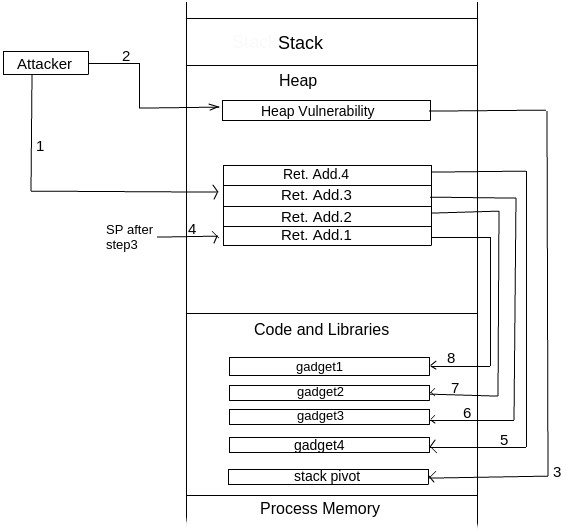
\includegraphics[scale=.40]{rop.jpg}\break purpose. Then the vulnerability present is exploited (say the buffer is overflown to overwrite the return address or, the address of code pointer is overwritten to point to stack pivot sequence)(step2). It directs the control to the stack pivot sequence when the exploited vulnerability is used by the application(step3). The stack pivot sequence modifies the stack pointer(\%esp) value to direct it to the attackers payload. After the execution of the stack pivot sequence the stack pointer now points to the Ret.Add.1 that points to gadget1(step4). The "ret" instruction at the end loads the address pointed to by stack pointer in the instruction pointer and increments the stack pointer by 1. Now, gadget1 is executed and the stack pointer has been incremented to point to Ret.Add.2 that points to gadget2(step5). It goes on incrementing the stack pointer and executing the gadgets until the goal is reached.
	
	\subsection{Basic Mitigation Techniques}
	The security researchers have proposed many method over last few years but the two leading defensive techniques against code-reuse attacks are control-flow integrity and address space layout randomisation. Overview of these techniques is given below.
	
	\subsubsection{Control-flow Integrity}
	One of the important step in any code-reuse approach is to alter the control flow of the application to direct it to the attacker payload. This approach prevents the attack by taking care of the control flow of the application. It creates a control flow graph(CFG) of the application before execution. Each node of CFG represents a basic block i.e., a straight piece of code in which there are no jumps to any location, with two special blocks, the entry block where control enters the CFG and the exit block through which control flow leaves CFG. CFG generally represents all the possible paths that can be traversed by the program during its execution. In CFI policy, the runtime behaviour of the application is monitored to ensure that a valid path is followed by the control flow in CFG. If it deviates from valid path then a CFI exception is raised and the application is terminated. Thus, the attacker can not alter the control flow of the application. But, enforcing this policy has performance issues. As, checking all indirect control flow transfers has a high performance impact like checking the function returns using a shadow stack increases the overhead by 21\%. Shadow stack is similar to the call stack and stores the return addresses which are compared with when the functions return. So, this approach is not widely accepted.
	
	Several coarse-grained CFI policies have also been proposed to overcome the shortcomings of the original CFI policy. These coarse-grained policies relaxes the original CFI policy and allows additional execution paths beyond those intended by the programmer. The original CFI polices ensures that the return address points only to the original caller by comparing return addresses using shadow stack. But, coarse-grained CFI policies relaxes it by checking only that the return address points to an instruction directly after a call instruction. Some methods use heuristics for prevention like they monitor the number of instruction executed between consecutive branches i.e., trying to detect the number of short execution sequences of the ROP technique. But, it has been shown that using a commonly used system library on windows an attacker can still craft a Turing-complete gadget set and perform code-reuse attack. And has also developed a new gadget called long-NOP that increases the length of each gadget by adding some instruction that would not alter the behaviour required by attacker, thus it bypasses the heuristics approach that checks the number of short instruction sequences \cite{effcfi}.
	
	\subsubsection{Address Space Layout Randomisation}
	The exploitation techniques overwrites the return address in order to point to the payload inserted by the attacker. ASLR does not remove these vulnerabilities instead it makes them more difficult to exploit by randomising the address space for each instantiation of the program. The basic idea of ASLR is to randomise the base address of all the process areas like text, data, bss, libraries, etc.
	
	In order to craft the attack the attackers need to know the address of the code sequences that they would use as gadgets. The address layout being randomised attackers need to guess the address. Thus, security of ASLR is based on the chances of the attacker guessing the addresses of the areas which are randomly placed by ASLR. The initial ASLR implementations mostly focussed on randomising the libraries only, which was able to prevent the return-to-libc attacks as the address of libc was randomised. But, the advent of ROP increased the need of full implementation of ASLR, as ROP can use code from any non-randomised section to craft the attack.
	
	ASLR is also suppored by Microsoft Windows starting from Windows Vista and all later versions. Apple included it from Mac OS X v10.5. The linux PaX project \cite{pax} in 2001 presented the most complete implementation of ASLR providing most entropy for each randomised layout as compared to other implementations. PaX applied ASLR to ELF binaries and shared libraries. It randomised the area of process's user address space splitting it in three groups i.e., the executable area that includes executable code, initialized and uninitialised data, the stack area that contains the user stack, and the mapped area including dynamic libraries and heap. For this a random offset is chosen and added to base address of these areas (different offset for different area) each time the process is created. It provides entropy of 16, 24, and 16 bits for executable area, stack area, and mapped area, respectively.
	
	But, ASLR suffered from two main issues, first the entropy of 32-bit is too low and second it is vulnerable to memory discloser attacks i.e., even if a single pointer is leaked it may lead to the failure of whole ASLR. It has been shown that ASLR on $\times$86 architecture can be bypassed by brute force \cite{effaslr} and proposed the migration to 64-bit ASLR that gives an entropy of 28-bits to mapped area. To prevent this many fine-grained ASLR schemes were proposed. The main idea in these was to randomise the data and code structure including the basic blocks and functions. Thus, even if a single address is leaked it would no longer makes code reuse attack feasible. But, some scheme came into existence that can defeat even the fine-grained ASLR \cite{jitrop}.
	
	The shared libraries are common to the processes using them. So, they are generally not randomised along with creation of each process in order to get the benefit of sharing. So, these libraries are generally randomised as per boot basis i.e., each time system boots a random offset is added to the base, and it is used as it is for the rest of the time. Microsoft windows follows this approach. But the ASLR implementation of Linux is more advanced. It compiles libraries as position independent code(POC) which allows it to share the same executable image of library among several processes and each one can map it according to themselves at different address. Rather than working on absolute addresses the POC code works with relative offsets to the program counter. The code of application when compiled as position independent is called Position independent executable(PIE), which is similar to PIC in principle. But, bypass of ASLR on 64-bit is shown when executable are PIE compiled using a offset2lib vulnerability \cite{effaslr64}. This exploit relies on the fact that when an application is PIE compiled the distance in bytes from where application was loaded and where the libraries are mapped is same for all executions of the application on a system. As the ASLR algorithm of Linux loads the first ASLR object at random location and loads the next just below it. This offset depends on the size and number of libraries in between and are different depending on system, But are unchanged between different execution of the same application. It also offers a solution to remove this offset2lib weakness by creating a different zone for the executable.
	
	Several methods to prevent address leakage on ASLR are also proposed like ASLR-Guard \cite{aslrguard}. ASLR-Guard prevents ASLR by completely preventing the leak of code locator. Code locators refers to any pointer or data that can be used to get code address. It divides the process address space into two sections data section and code section. And acts as a gateway between these two sections. Whenever a code address is leaked to the data section it encrypts the address as a token and decrypts the token whenever the token is used to perform control transfer. Thereby, preventing all explicit code locator leaks.
	
	\section{Advanced Offensive and Defensive Techniques}
	Although many defensive solutions have been proposed but there are many methods that can bypass these solutions. Some advanced techniques like just-in-time code reuse \cite{jitrop} and the method shown by Davi et al. \cite{effcfi} can bypass the fine-grained ASLR and the CFI techniques, respectively. Also there are some advanced defensive methods proposed like HAFIX \cite{hafix} which is hardware based solution and Isomeron which prevents attack by randomising the control flow using two isomers for each function, one retains the layout and other is modified and it determines randomly whether a return should switch execution to other isomer or continues on same isomer.
	
	Here, we describe one offensive just-in-time Code Reuse \cite{jitrop} method and one defensive the HAFIX \cite{hafix} method.
	
	\subsection{Just-In-Time Code Reuse(Offensive)}
	Just-In-Time Code Reuse uses the return oriented programming technique(JIT-ROP). It assumes the presence of normal defensive mechanisms on the target platform like NX bit and also assumes the deployment of fine-grained ASLR i.e., randomisation is done even at the basic block level. It just need any memory address at runtime from the process address space unlike others that needs the address layout. This address can be easily obtained by exploiting a memory vulnerability. It generates the gadgets recursively at runtime using the disclosed memory address.
	
	The initial step is to exploit a memory vulnerability to get a memory address. Then, this address is used to obtain the memory layout of the process. We know that the page size is 4KB and the disclosed address would reside in a memory page. So, the starting and ending address of that page can be determined. JIT-ROP requires exploit writer to conform that disclosed address to an interface called Disclosebyte that discloses the one byte of data present at that address. This is used to disclose the whole memory page. Thus, upon disassembling the page obtained we got a 4KB space that would be used to create gadgets. This disassembled page would also contain direct branches to other pages like call instructions. So, by using that branch address other page can also be disassembled just like the previous page. similarly, other pages can be obtained and the process goes on until no new direct branches to undisclosed pages are obtained. The memory pages disclosed are used to find the gadgets at runtime using Galileo algorithm by iterating over the pages. These gadgets are verified and only those which meet the gadget semantic definitions are accepted i.e., the gadgets which don't have any side-effect like modifying the stack pointer. All of this is done at runtime. After obtaining all the gadgets required, the ROP payload is constructed and proceeded like normal ROP attack.
	
	\subsection{HAFIX: Hardware-Assisted Flow Integrity Extension(Defensive)}
	The software-based fine-grained CFI approaches incurs high performance overheads. And the coarse-grained approaches are also shown to be bypassed. HAFIX is a hardware based Backward-edge CFI approach implemented on SPARC and Intel Siskiyou architecture and incurs a overhead of 2\%, much better than other CFI approaches. Backward-edge CFI approach means it focus on return instructions instead of calls and jumps. The idea used in HAFIX is to confine function returns to active call sites i.e., a return instruction is allowed to only target a call preceded instruction in a function that is currently active. This policy needs a little modification in the compiler and can be easily implemented in hardware.
	
	HAFIX requires the compiler to assign a unique label to each function and also the first instruction to be CFIBR. This instruction loads the function label into a dedicated memory called label state memory. The label remains in the label state memory as long as the function is active. Any direct or indirect call leads to a change in processor state where only the CFIBR instructions are accepted. And CFIDEL instruction is used to remove the label from the label state memory. Since, HAFIX allows return to only active call sites so only those CFIRET instructions are permitted which define a label in the label state memory, otherwise a CFI exception is raised.
	
	In order to handle recursive calls it introduces a new CFI instruction CFIREC and a new shadow register CFIREC\_CNTR. At the starting of a recursive function instead of CFIBR the compiler emits a CFIREC instruction that puts label in label state memory and sets the CFIREC\_CNTR to zero. It also increments CFIREC\_CNTR on subsequent recursive calls. Also the label is internally associated with the CFIREC\_CNTR register. When function returns the CFIDEL checks whether the current label is associated with CFIREC\_CNTR if so then CFIREC\_CNTR is decremented and is removed from label state memory only when it is equal to 1 indicating that the last instance of recursive function has returned.
	
	\section{Defences using Recompilation and Code-Rewriting}
	These defences are compiler-based approaches to defeat return oriented programming. These depends on recompilation of the binaries to removed the code sequences from the binaries that can be used as gadgets by attacker for building ROP payload.
	
	Jinku Li et al.\cite{kernel} that proposed return-less kernel by entirely removing the opcode of \textit{ret} instruction from all instructions and G-Free by Kaan Onarlioglu et al.\cite{gfree} that makes gadgets with \textit{ret} instructions almost impossible to use by removing unintended \textit{ret} instructions and encrypting the return addresses.
	
	\subsection{Return-less kernel Approach}
	The main focus of this approach is the removal of the opcode of \textit{ret} from the code so that no ROP gadgets can be crafted. To remove the \textit{ret} opcode generated by \textit{ret} instruction itself a centralized return address table is maintained to store the return addresses of the functions. When a call is made its execution is instrumented to push a return index instead of return address on the stack. And when a \textit{ret} is executed instead of poping a return address from stack its execution is instrumented to take the return index and use it to get return address form the centralized return address table and transfer the control flow. To remove the \textit{ret} opcodes generated from register usage the compiler register allocation is adjusted. For example, the instruction \textit{mov \%rax, \%rbx} has machine code \textit{48 89 c3} so, \textit{rbx} register needs to be replaced with some other register as it is the one introducing \textit{c3} byte. The other sources are instructions that contain \textit{ret} opcode in their opcodes or immediate operands for these peephole optimization is used.
	
	This approach has been proposed specially for gadget-less kernel compilation and exploits characteristics of kernel code for removal of gadgets and has performance overhead. It also requires manual modifications in the assembly routines.
	
	\subsection{G-Free Approach}
	G-Free is a compiler based recompilation approach that removes all unaligned branch instructions from a binary executable and prevents aligned free-branch instructions from being misused. Its working can be divided into two sets.
	
	The first set protects the aligned free-branch instructions that are present in the executable. These instructions are \textit{ret} instructions and \textit{call}/\textit{jmp} instructions that directly changes the control flow of program. The functions are instrumented with small code blocks to ensure that if the executing function has been entered from its proper entry point only then the aligned free-branch instructions can be executed. In particular two complementary techniques are employed: return address encryption for protecting \textit{ret} instructions and cookie-based technique which is applied only to functions with \textit{call}/\textit{jmp} instructions.
	
	The return address protection instruments entry points of the function with header that encrypts
the saved return address stored on the stack and corresponding footer before \textit{ret} instruction to restore the return address to its original value. So, if the attacker jumps into a function at an arbitrary position and eventually reaches the footer, decryption routine would process the unencrypted return address provided by the attacker resulting in invalid value and transfers the control to that incorrect address, on which the attacker would have no control.

	To prevent \textit{call}/\textit{jmp} instructions, the functions with these instructions are instrumented with additional header that compute and push a random cookie on the stack. The cookie is \textit{XOR} of random key generated at runtime and per-function constant generated a the compile time which is used to uniquely identify the functions. The \textit{call}/\textit{jmp} instructions are prepended with a validation block that fetches cookie, decrypts it, and compares with the per-function constant. The application is crashed if the values does not match.
	
	The second set does code rewriting to remove all unaligned free-branch instructions. In IA-32 a \textit{ret} instruction can be encoded with any of 0xc2, 0xc3, 0xca, or 0xcb bytes and can be part of any field of any instruction. The \textit{call}/\textit{jmp} instructions are encoded as 0xff follwed by ModR/M byte carrying some 3-bit sequence, so instead of appearing inside a single instruction, it can also be obtained by a combination of two bytes from two consecutive instructions. For example, an instruction like \textit{movl \%eax, \%ebx} assigns value 0xc3 to the ModR/M byte. So, when these instructions are detected the compiler register allocation stage can be performed again with a different register assignment. Alternatively, the register contents can be swapped with some other register and the instruction can be rewritten with that register as operand.
	
	G-Free removes all unaligned free-branch instructions from a binary and protect the aligned ones but does not remove the free branches so the attacker can directly jump into the protection blocks and reach the free branch instructions. Also, it includes instrumenting the functions with protection code that incurs overhead.

	\section{An example using Return Oriented Programming}
	The following example is performed just to show the working of ROP attack. Tool Ropeme\cite{ropeme} is used for finding gadgets(including stack pivot) required for building ROP payload. Performed on Ubuntu 12.04 LTS, with stack canary protection and ASLR turned off.\break Stack canary can be turned off using the gcc flag \textit{-fno-stack-protector} while compilation and,\break ASLR can be disabled by the command \textit{echo 0 $<$ /proc/sys/kernel/randomize\_va\_space} in terminal by \textit{sudo} user. 
	
	Consider the vulnerable program in the figure below
	\break \break
	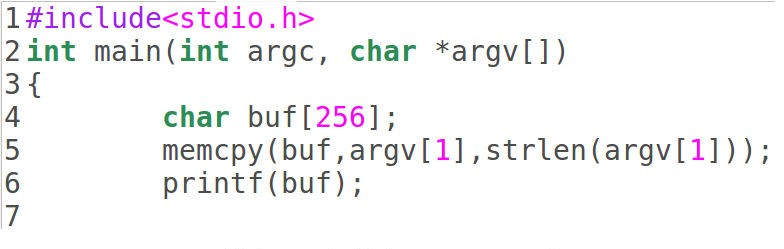
\includegraphics[scale=.27]{vul_prog.jpg}\break \break
	The program contains a buffer overflow vulnerability at the array \textit{char buf[256]}, bound checking is not performed before copying data to this array. So, this array would be made to overflow and write to the locations beyond its limit, which in turn overwrites the return address by the address of the stack pivot gadget. Thus, when the function returns it would return to the stack pivot gadgets and execute it. The stack pivot will modify the stack pointer to point it to the payload and the execution of the payload starts.
	
	Consider the below input to the program - \break
	`python -c 'print "A"*264+"\textbackslash x5e\textbackslash x15\textbackslash xe5\textbackslash xb7"+ "\textbackslash xa1\textbackslash xe5\textbackslash xe9\textbackslash xb7"+"\textbackslash x4f\textbackslash x40\textbackslash xe4\textbackslash xb7"+ $\ldots\ldots$ + "\textbackslash xb0\textbackslash xf1\textbackslash xfd\textbackslash xb7"'` \break
	The A's fills the stack till the return address and the return address is overwritten with 0xb7e5155e which is the address of the stack pivot gadget \textit{"add esp} 0x4;\textit{ ret"} which when executed increments the stack pointer(\%esp) by 4. So, now when the function returns it returns to 0xb7e5155e which is the address of the stack pivot gadget. And the remaining data is copied over on stack. The 2nd address is the address of a \textit{NOP} gadget which will not do any operation and simply increments the pointer to point to the next gadget. The actual ROP payload starts from 0xb7e4404f which is the 3rd address in the given input so we need to make the stack pointer to point to 3rd address in input. The address of the gadgets in the payload are given in the little-endian format as per the requirement of the system. After the function returns, the stack pointer would initially point to the address of \textit{NOP} gadget because it is the one present next to the return address on the stack and when the stack pivot is executed it increments the stack pointer by 4 which makes stack pointer to point to the ROP payload. So, now the payload executes and pops up a shell upon completion.
	
	\section{Proposed Defensive Technique}
	The success of any code-reuse attack depends on the discovery of the suitable gadgets. Consider the Return-oriented programming attack which executes the ROP payload consisting of ROP gadgets. The payload can be loaded to any attacker suitable location like heap, stack, etc. In order to execute the payload the attacker needs to direct the control flow of the program to the payload, which is usually done by modifying the stack pointer(\%esp) and making the stack pointer to point to the starting of payload. And this task is performed by the stack pivot sequence.
	
	The basic idea of the proposed approach is to prevent the discovery of these stack pivot sequences. For which these sequences are replaced with some other assembly code and replaced back upon execution.
	
	\subsection{Model}
	To prevent the exposure of stack pivot sequences these and replaced with some dummy assembly code in the executable and stored, so the attacker would not be able to find that he could have been able to before replacement. Before execution the original code is replaced back at correct position in the executable. The process basically includes two phases- first one the encryption phase and second the decryption phase.\break
	
	\subsubsection{First Phase}
	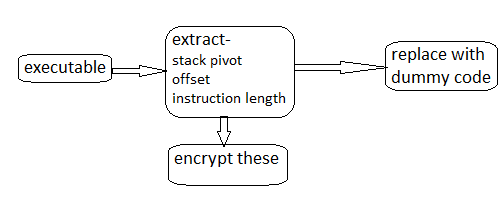
\includegraphics[scale=.5]{phase1.png}\break
	The encryption phase deals with the form in which the executable is stored on the system. Initially, using a tool like Ropeme\cite{ropeme}, the executable to be secured is searched for the gadgets which are candidates for stack pivot sequences that can be used by the attacker and these gadgets are stored in a separate file. The information that would be required for placing them back like their offset from starting address and the length of the gadget are also stored in a file. These files are encrypted and kept at a secure location. The found stack pivots are now searched in the executable and are replaced with a dummy assembly code of same length as of the gadget being replaced. The executable is now available in the system in the form where the candidates for stack pivot are replaced by some other code. If the attacker now tries to search for stack pivots in that executable he would not be able to find any candidate. So, even if the attacker has placed the payload somewhere in process address space he won't be able to execute that payload as he don't have any stack pivot to direct control to the payload.
	
	\subsubsection{Second Phase}
	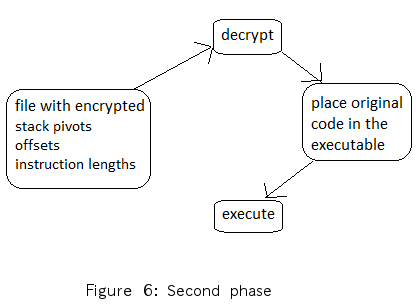
\includegraphics[scale=.5]{phase2.png}\break
	The executable after going through the first phase would not be able to execute in its normal way as some of its instructions have been modified. So, in order to execute normally the executable has to be converted back to as it was before going through the first phase. And this is the job of the second phase. To achieve this, first the encrypted files containing the stack pivots, offsets and instruction lengths are decrypted. Using the offset of a particular stack pivot sequence it is placed in its right place in the executable, and this is done for all stack pivots obtained from the first phase. After this has been done the executable is now the way it was before first phase and can now be executed normally.
	
	\subsection{Implementation Details}
	The approach is implemented only for offline purpose for the security of the stored files. so that no offline disclosure of gadgets is possible. It has been implemented on ubuntu 12.04 LTS using gcc 4.6.3 compiler. \break Three files other than the executable to be secured are maintained. These are as follows
	\begin{itemize}
		\item \textit{locations file} for storing the stack pivots found from the tool Ropeme\cite{ropeme}.
		\item \textit{len\_off file} for storing the length and offset of all instructions replaced in the executable.
		\item \textit{data file} for storing the instructions replaced in the executable.
	\end{itemize}
	Initially, the executable is scanned for stack pivots using the tool Ropeme\cite{ropeme} and the generated output is stored in the \textit{locations file}. Below is a sample output on a custom shared library we used for evaluation of approach that shows some stack pivot candidates along with offset from the starting address.\break \break
	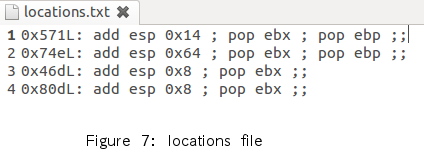
\includegraphics[scale=.55]{locations.png}\break
	After this, these gadgets are searched in the executable using the offset. And the binary data at those locations is copied to \textit{data file} and the length of the data copied and the offset are saved in \textit{len\_off file}. Below is a sample output of contents of the \textit{data file}.\break \break
	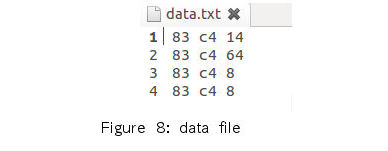
\includegraphics[scale=.5]{data.jpg}\break
	The \textit{locations file} can be removed from system after the first phase. And the others the \textit{data file} \& \textit{len\_off file} are encrypted using \textit{ccrypt} which is based on the Rijndael block cipher, a version of which is also used in the Advanced Encryption Standard(AES).
	
	After this, Ropeme\cite{ropeme} is again run to find stack pivots, but it was not able to find those gadgets that it found previously.
	
	In order to execute the executable it is converted back to its original form. First the \textit{data file} and \textit{len\_off file} are decrypted. Now using the offset and length information from \textit{len\_off file} the data from \textit{data file} is placed in its original location. And the executable now can be executed normally.
	
	\subsection{Security Evaluation}
	After encryption trying to find stack pivots results in nothing i.e., it is not able to find the stack pivots that it found initially. Also, the security of approach depends on the security of the key used for encryption and \textit{ccrypt} utility, which is used for encryption of the files. Also the key need to be stored on a secure location that cannot be accessed by any unauthorized means.

	\section{Conclusions and Future Work}
	Code-reuse attacks are one of the major exploits for a long period. Many studies have been done and approaches have been proposed to mitigate these attacks \cite{breakdef}\cite{secrvw}\cite{memerr}\cite{marlin}. Major approaches include stack canary, NX bit, Address space layout randomisation and control flow integrity checking. But, it has been shown time to time that these approaches can be bypassed. These exploits can not be prevented in a single moment, thus a fast progress towards mature security defences and towards the use of safe languages is required.
	
	To contribute to the current efforts we have proposed a method of mitigating code-reuse attacks by preventing the discloser of stack pivot sequences that are used by the attackers to direct the control flow to the exploit payload. The approach has been found to successfully prevent the disclosure of stack pivot sequences in a executable if that executable has been treated with the this approach.
	
	This approach has been implemented only in offline mode i.e., only the executables stored on disk can be encrypted by this and executed independently. To get it working online the files can be kept encrypted with this approach but it would need modification in loader that may incur some overhead, thus this can be taken as future work. One more modification that can be done is to keep signals in place of stack pivots and the stack pivots in the signal handler in encrypted form. So upon receiving signal from the process the stack pivots can be decrypted and executed on demand. But it would also need some OS level modifications and can be taken as future work.
	
    \bibliographystyle{abbrv}
    \bibliography{ref}
	
	\end{multicols}
\end{document}

% also cite ccrypt and Ropeme
